\documentclass[a4paper]{amsart}

\usepackage{color}
\usepackage[colorlinks=true, citecolor=red]{hyperref}  %needs to come before amsrefs package to work with \cite{}*{}
\usepackage{amssymb,latexsym}
\usepackage[alphabetic]{amsrefs}
\usepackage[mathscr]{eucal}
\usepackage{pdfsync}
\usepackage{graphicx}
\usepackage{epstopdf}
\DeclareGraphicsRule{.tif}{png}{.png}{`convert #1 `dirname #1`/`basename #1 .tif`.png}
\usepackage[all]{xy}
\usepackage{titletoc}

\CompileMatrices

\theoremstyle{plain}
\newtheorem{theorem}{Theorem}[section]
\newtheorem{lemma}[theorem]{Lemma}
\newtheorem{proposition}[theorem]{Proposition}
\newtheorem{corollary}[theorem]{Corollary}

\theoremstyle{definition}
\newtheorem{definition}[theorem]{Definition}%[section]

\theoremstyle{remark}
\newtheorem{example}[theorem]{Example}
\newtheorem{remark}[theorem]{Remark}
\newtheorem{discussion}[theorem]{Discussion}
\DeclareMathOperator{\Lip}{Lip}
\DeclareMathOperator{\dist}{dist}
\DeclareMathOperator{\expected}{\mathbb{E}}
\DeclareMathOperator{\prb}{Prob}
\DeclareMathOperator{\spt}{spt}
\DeclareMathOperator{\lap}{\Delta}

\raggedbottom

\addtolength{\textwidth}{2cm}
\addtolength{\oddsidemargin}{-1cm}
\addtolength{\evensidemargin}{-1cm} 
\addtolength{\topmargin}{-1cm} 
\addtolength{\textheight}{2cm}
% \renewcommand{\l@subsection}{\@contentsline{2}{5em}{7em}}

%\makeatletter
%\makeatother

 
%%% BEGIN DOCUMENT
\begin{document}

\title{Convolution, Characteristic Function, Fourier transform}  
\author{John E.\ Hutchinson}
\date{\today}

\maketitle


%\renewcommand*\l@subsection{\@tocline{4}{50em}{7em}{10em}{10em}}


\tableofcontents

%%%%%%%%%%%%%%%%%%%%%%%%%%%%%%%%
%%%%%%%%%%%%%%%%%%%%%%%%%%%%%%%%
%%%%%%%%%%%%%%%%%%%%%%%%%%%%%%%%
%%%%%%%%%%%%%%%%%%%%%%%%%%%%%%%%
\section{\textbf{Convolution Interpretation}} 
I follow~\cite{Fol}*{p 207} 

\medskip From the definition
\begin{equation} \label{dfcon} 
(f*g)(x) = \int  f(x-y) \, g(y)\, dy = \int f(y)\, g(x-y) \, dy,
\end{equation} 
one has two interpretations.

In both cases think of $ f $ as the ``main'' function and $ g $ as the subsidiary ``weighting'' or ``mollifying'' function.

%%%%%%%%%%%%%%%%%%%%%%%%%%%%%%%%
\subsection{Linear Combination of Translates}
From the first integral in \eqref{dfcon}, using Riemann sums:
\[
(f*g)(x)  = \int  f(x-y) \, g(y)\, dy \approx \sum_i f(x-y_i)\, g(y_i) \Delta y_i .
\]
So 
\begin{gather} \label{} 
\text{ \parbox{4.2in}{ \emph{The \underline{function}  $ f *g$ is the continuous superposition (linear combination) of translates of $ f $ by $ y_i $ with coefficients $ g(y_i)\Delta y_i $.}}} 
\end{gather} 


%%%%%%%%%%%%%%%%%%%%%%%%%%%%%%%%
\subsection{Weighted Average}
From the second  integral in \eqref{dfcon},
\[
(f*g)(x)   = \int f(y)\, g(x-y) \, dy.
\]
Consider the case $ g \geq 0 $ and $ \int g= 1 $.  
Then 
\begin{gather} \label{} 
\text{ \parbox{2.7in}{
\emph{The \underline{value}   $(f*g)(x) $  is the weighted average of $ f $ using the weight function  $ w(\cdot) = g(x-\cdot) $}.}}
\end{gather}
The weight function $g(x-\cdot) $  is obtained from $ g $ by reflecting the graph of $ g $ in the vertical axis and then translating by $x $.  See Figure~\ref{convol}.

\begin{figure}[htbp] %  figure placement: here, top, bottom, or page
   \centering
   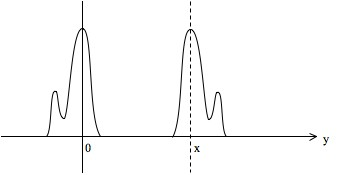
\includegraphics[width=3in]{convol.jpg} 
   \caption{The graph of $ y\mapsto g(y) $ is on the left  and the graph of $ y\mapsto g(x-y) $ is on the right.}
   \label{convol}
\end{figure}

For example, if 
\begin{gather*}
 g = \frac{1}{2a} \mathcal{X}_{[-a,a]}, \quad g(x-\cdot) = \frac{1}{2a} \mathcal{X}_{[x-a,x+a]} (\cdot), \\ 
\text{then} \quad (f*g)(x) = \frac{1}{2a}\int_{x-a}^{x+a} f .
\end{gather*}





%%%%%%%%%%%%%%%%%%%%%%%%%%%%%%%%
%%%%%%%%%%%%%%%%%%%%%%%%%%%%%%%%
%%%%%%%%%%%%%%%%%%%%%%%%%%%%%%%%
%%%%%%%%%%%%%%%%%%%%%%%%%%%%%%%%




\section{\textbf{Fourier transform of nice function}}

I follow \cite{CH}*{pp 77--79}.

\subsection{Motivation for inversion formula}
Suppose $ f \in L^1(\mathbb{R}) $,   continuous and piecewise $ C^1 $.

\medskip
The Fourier series on $ [-L,L] $ is 
\begin{align*}
f(x) &= \sum_{n=-\infty}^{n = \infty} a_n e^{in\frac{\pi}{L} x},  \\
a_n &= \frac{1}{2L}\int_{-L}^L f(t) e^{-in\frac{\pi}{L} t}\, dt .
\end{align*}
(Convergence is both pointwise and in $ L^2 $ sense.)

 
Hence on $ [-L,L] $,
\[
f(x) = \frac{1}{2\pi} \sum_{n=-\infty}^{n = \infty}  \frac{\pi}{L} \int_{-L}^L f(t)  e^{in\frac{\pi}{L}( x-t)}\, dt .
\]

Let $ L\to \infty  $ and thinking of $ \pi/L $ as $ \delta u $ it is \emph{plausible} that 
\begin{align}
f(x) &= \frac{1}{2\pi}  \int_{-\infty}^\infty  \left(  \int_{-\infty}^\infty f(t) e^{iu(x-t)} \, dt \right) \, du  \notag\\
& =   \frac{1}{2\pi}  \int_{-\infty}^\infty  \left(  \int_{-\infty}^\infty f(t) e^{-iut} \, dt \right) e^{iux} \, du.  \label{ft1}
\end{align}


\medskip
The \emph{Fourier transform} is defined by 
\[
\widehat{f} (u) :=  \int_{-\infty}^\infty f(t) e^{-iut}\, dt,
\]
and so we can write \eqref{ft1} as  the inversion formula
\begin{equation} \label{ft2}
f(x) = \frac{1}{2\pi}  \int_{-\infty}^\infty  \widehat{f} (u) e^{iux}\, du.
\end{equation} 


%%%%%%%%%%%%%%%%%%%%%%%%%%%%%%%%%%%%
\subsection{Proof of inversion formula}

Instead of rigorously justifying the limit used to obtain \eqref{ft1} it is easier to prove  \eqref{ft1} directly as follows.

\begin{proof}
\begin{align}
f(x) &= \lim_{v \to \infty} \frac{1}{\pi} \int_{-a}^a f(x-t)\frac{\sin vt}{t}\, dt \label{ft3} 
\intertext{($ \frac{\sin vt}{t} $ is essentially the Dirichlet kernel -- give reference ***)}
&=  \lim_{v \to \infty} \frac{1}{\pi} \int_{-a}^a f(x-t)   \left( \int_0^v \cos ut \, du \right)    dt  \notag\\
&=  \lim_{v \to \infty} \frac{1}{\pi} \int_0^v \left( \int_{-a}^a f(x-t) \cos ut \, dt \right)   du  \notag\\
&=     \frac{1}{\pi} \int_0^\infty \left( \int_{-a}^a f(x-t) \cos ut \, dt \right)   du  \notag \\
&\to   \frac{1}{\pi} \int_0^\infty \left( \int_{-\infty}^\infty f(x-t) \cos ut \, dt \right)   du \quad   \text{as } a \to \infty \notag
\intertext{(since using \eqref{ft3} the error is bounded by $ \frac{1}{2\pi a} \| f \|_{L^1}$  )} 
 &=   \frac{1}{2\pi} \int_{-\infty}^\infty \left( \int_{-\infty}^\infty f(x-t) e^{iut} \, dt \right)   du    \notag
 \intertext{(since $ \sin ut $ is odd in $ u $)}
 &=   \frac{1}{2\pi} \int_{-\infty}^\infty \left( \int_{-\infty}^\infty f(t) e^{iu(x-t)} \, dt \right)   du    \notag
\end{align} 
 This is \eqref{ft1}.
\end{proof} 



%%%%%%%%%%%%%%%%%%%%%%%%%%%%%%%%%%%%%%
%%%%%%%%%%%%%%%%%%%%%%%%%%%%%%%%%%%%%%%%
%%%%%%%%%%%%%%%%%%%%%%%%%%%%%%%%%%%%%%%%%%
\section{\textbf{Characteristic Function}}

I follow \cite{Ash}*{pp 291--298}

\subsection{Definitions}
Suppose $ \mu $ is a probability measure (more generally, a finite measure)  on $ \mathcal{B}(\mathbb{R}) $.

The \emph{probability distribution} $ F $ is defined either as a measure or as a function by
 \[
\mu(a,b] = F(a,b] = F(b) - F(a).
\]
So $ F $ is increasing, continuous from the right, and has a limit from the left.

 
\medskip
The \emph{characteristic function} $ h  $ is
\begin{equation} \label{} 
h(u) = \int e^{iux}\,  d\mu (x)  = \int e^{iux} \, dF(x) = \mathbb{E} e^{iuX} ,
\end{equation} 
where in the last term, $ X $ is any r.v.\ with $ \dist X  = F $.

If $ F $ is $ C^1 $ this is just the Fourier transform of the corresponding probability density $ dF/dx$    with a sign change.


%%%%%%%%%%%%%%%%%%%%%%%%%%%%%%%%%%%%%%%%
\subsection{Inversion formula}  
\begin{proposition}
Suppose $ h $ is the characteristic function of the distribution $ F $, and suppose $ h \in L^1 $.  Then
\begin{equation} \label{ft4}
f(x) := \frac{1}{2\pi} \int_{-\infty}^\infty e^{-iux} h(u)\, du
\end{equation}
is a density for $ F $.  

One \emph{always} has (without assuming $ f \in L^1$)
\begin{equation} \label{ft5}
F(a,b] = \lim_{c\to \infty} \frac{1}{2\pi} \int_{-c}^c \frac{e^{-iua} - e^{-iub}}{iu} h(u) \, du ,
\end{equation} 
if $ F $ is continuous at $ a $ and $ b $.
\end{proposition} 

\emph{Remark}: Formally, \eqref{ft5} comes from \eqref{ft4} by integrating.  But it holds more generally.

\begin{proof}
Let
\begin{align*}
 I_c &= \frac{1}{2\pi} \int_{-c}^c \frac{e^{-iua} - e^{-iub}}{iu} h(u) \, du \\
      &=  \frac{1}{2\pi} \int_{-c}^c \frac{e^{-iua} - e^{-iub}}{iu} \left( \int_{-\infty}^\infty e^{iux} \, dF(x)\right) du  \\
      &=  \frac{1}{2\pi}  \int_{-\infty}^\infty \left( \int_{-c}^c \frac{e^{-iua} - e^{-iub}}{iu}\,  e^{iux} \, du \right) dF(x)  \\     
      &=  \frac{1}{2\pi}  \int_{-\infty}^\infty \left( \int_{-c}^c \frac{\sin u(x-a) -\sin u(x-b)}{u}  \, du \right) dF(x)   
      \intertext{(the ``$  \cos $ part'' is odd and so integrates to $  0 $)}    
      &=  \frac{1}{2\pi}  \int_{-\infty}^\infty \left( 
                     \int_{-c(x-a)}^{c(x-a)} \frac{\sin v}{v}  \, dv  -  \int_{-c(x-b)}^{c(x-b)} \frac{\sin v}{v}  \, dv\right) dF(x).         
\end{align*} 
Since $ \int_{-\infty}^\infty \frac{\sin v} {v}\, dv = \pi $, as $ c \to \infty $, the inner term converges to $ 2\pi \mathcal{X}_{(a,b]} + \pi  \mathcal{X}_{\{a\}} - \pi \mathcal{X}_{\{b\}} $, 
. By the D.C.T.\ 
\[
I_c \to F(a,b] + \frac{1}{2} f\{a\} -\frac{1}{2} f\{b\} ,
\]
proving a bit more than stated in \eqref{ft5}.

\medskip
Next assume $ h $ is integrable.  

Then $ f $ \emph{defined} by  \eqref{ft4} is \emph{continuous} by the D.C.T.  

Moreover
\begin{align}
\int_a^b f(x)\, dx   &=  \frac{1}{2\pi} \int_{-\infty}^\infty h(u) \left( \int_a^b e^{-iux} dx \right) du \notag \\
&= \lim_{c\to \infty} \int_{-c}^c h(u) \frac{e^{-iua}- e^{-iub}}{iu}\, du \notag\\
&= F(a,b] , \label{ft6}
\end{align}
provided $ a $ and $ b $ are continuity points of $ F $ , i.e.\ $ F\{a\} = F\{b\} = 0 $.

Since the discontinuities of $ F $ are countable, the continuous points are dense.  It follows $ F\{c\} = 0 \ \forall c $, and so \eqref{ft6} is true for all $ a $ and $ b $.

It follows $ F $ is differentiable everywhere and $  F' = f $. 
\end{proof} 


%%%%%%%%%%%%%%%%%%%%%%%%%%%%%%%%%%%%%%%
\subsection{Properties of the characteristic function}


\begin{enumerate} 

\item Suppose $ S = X_1 +\cdots X_n $ where the $ X_i $ are independent with characteristic function $ h_i $. Then $ S $ has characteristic function $ h = h_1 \times \dots \times h_n $.

 \emph{Proof}: $ \mathbb{E} e^{iu(X_1 + X_2)} = \mathbb{E} e^{iu X_1   }   \mathbb{E} e^{iu  X_2 } $ by independence.

\item $  |h(u)| \leq h(0) = 1 $.

\emph{Proof}: Immediate 

\item $ h $ is continuous.

\emph{Proof}: By D.C.T. 

\item $ h(-u) = \overline{h(u)} $.

\emph{Proof}: Immediate.


\item $ h $ is real valued if $ F $ is symmetric. (In fact, ``iff'')

\emph{Proof}: Since $ \overline{h(u)} = \int e^{-iux}\, dF(x) = \int e^{ iux}\, dF(x) = h(u) $, where the second equality is by the symmetry. 

\item If $ \mathbb{E} |X|^k < \infty $ then $ h \in C^1 $, $ h^{(k)}(u) = \int (ix)^k e^{iux}\, dF(x) $,
h$ ^k(0) = i^k \mathbb{E} X^k$.

\emph{Proof}: The $ k=1 $ case follows from the D.C.T.\ after applying the mean value theorem.  Then use induction for $ k \geq 1 $. 

\item \emph{Bochner's Theorem}: $ h $ is a characteristic function iff $ h $ is continuous at $ 0 $ and   \emph{nonnegative definite}.  

That is,
$ \sum_{j,k=1}^n h(u_j-u_k) a_j \overline{a}_k $ is real and $ \geq 0 $ for all $ n $, all $ u_1,\dots, u_n \in \mathbb{R} $, and all $ a_1,\dots, a_n \in \mathbb{C} $.  

\emph{Proof}:   If $ h $ is a characteristic function it is continuous everywhere by (3).  Also
\[
0 \leq \int \bigg| \sum_{j=1}^n a_j e^{iu_j x} \bigg|^2 dF(x)= \sum_{j,k=1}^n \int a_j e^{iu_j x} \overline{a}_k e^{-iu_k x} dF(x)= 
                   \sum_{j,k=1}^n h(u_j-u_k) a_j \overline{a}_k.
                   \]
The other direction is non trivial.


\end{enumerate} 


%%%%%%%%%%%%%%%%%%%%%%%%%%%%%%%%%%%%%%%%%%%%%%%
%%%%%%%%%%%%%%%%%%%%%%%%%%%%%%%%%%%%%%%%%%%%%%%%%%
%%%%%%%%%%%%%%%%%%%%%%%%%%%%%%%%%%%%%%%%%%%%%%%

\begin{thebibliography}{9} 

\bib{Ash}{book}{
   author={Ash, Robert B.},
   title={Probability and measure theory},
   edition={2},
   note={With contributions by Catherine Dol\'eans-Dade},
   publisher={Harcourt/Academic Press, Burlington, MA},
   date={2000},
%   pages={xii+516},
%   isbn={0-12-065202-1},
%   review={\MR{1810041 (2001j:28001)}},
}


\bib{CH}{book}{
   author={Courant, R.},
   author={Hilbert, D.},
   title={Methods of mathematical physics. Vol. I},
   publisher={Interscience Publishers, Inc., New York, N.Y.},
   date={1953},
%   pages={xv+561},
%   review={\MR{0065391 (16,426a)}},
}

\bib{Fol}{book}{
   author={Folland, Gerald B.},
   title={Fourier analysis and its applications},
%   series={The Wadsworth \& Brooks/Cole Mathematics Series},
   publisher={Wadsworth \& Brooks/Cole},
%%   place={Pacific Grove, CA},
   date={1992},
   pages={x+433},
%%   isbn={0-534-17094-3},
%%   review={\MR{1145236 (93f:42001)}},
}
	
 
\end{thebibliography}





\end{document}


